\documentclass[11pt,a4paper]{article}

\usepackage[utf8]{inputenc}
\usepackage[T1]{fontenc}
\usepackage[margin=1in]{geometry}
\usepackage{graphicx}
\usepackage{amsmath}
\usepackage{xcolor}
\usepackage{listings}
\usepackage{hyperref}
\usepackage{enumitem}
\usepackage{tikz}
\usetikzlibrary{arrows.meta, positioning, shapes.geometric}

\hypersetup{
    colorlinks=true,
    linkcolor=black,
    urlcolor=blue!60!black,
    citecolor=black
}

% Code listings style
\definecolor{codebg}{rgb}{0.97,0.97,0.97}
\definecolor{codecomment}{rgb}{0.35,0.55,0.35}
\definecolor{codekey}{rgb}{0.15,0.15,0.6}
\definecolor{codestring}{rgb}{0.6,0.1,0.1}

\lstdefinestyle{default}{
    backgroundcolor=\color{codebg},
    basicstyle=\ttfamily\small,
    commentstyle=\color{codecomment}\itshape,
    keywordstyle=\color{codekey}\bfseries,
    stringstyle=\color{codestring},
    breaklines=true,
    breakatwhitespace=false,
    tabsize=2,
    captionpos=b,
    showstringspaces=false,
    frame=single,
    framesep=4pt,
    rulecolor=\color{gray!40},
    xleftmargin=6pt,
    xrightmargin=2pt
}
\lstset{style=default}

\lstdefinelanguage{puredata}{
    keywords={obj,msg,connect,canvas,text,restore,osc,dac,line,vline,noise,bp,hip,lop,route,unpack,pack,netreceive,oscparse,throw,catch,clip,r,s},
    sensitive=true,
    comment=[l]{\#},
    morestring=[b]"
}

\title{\textbf{MR~Drumset}\\[0.3em]
\large A Mixed-Reality Percussion Instrument with Dataflow Audio Synthesis}
\author{ Istrate Irina | Stancu Rares | Ioana Madalin | Jilavu Izabela | Manolachi George }
\date{April 2026}

\begin{document}
\maketitle

\begin{abstract}
\noindent
MR~Drumset is an interactive mixed-reality application that turns a
Pico~4 headset into an eight-piece percussion instrument. Three
independent processes cooperate over Socket.IO and OSC: a
WebXR/Three.js frontend rendering the instruments and detecting stick
collisions, a Node.js bridge forwarding hits as OSC messages, and a
Pure~Data patch that synthesises the sound using the dataflow
paradigm central to this course. The frontend additionally
doubles-renders on a desktop browser to produce a live spectator
mirror of the VR session. This report describes the architecture, the
swept-plane collision model used to get reliable hit detection on
arbitrarily oriented surfaces, the role of visual dataflow
programming in the audio engine, and the design trade-offs chosen to
hit the 72\,Hz performance budget of the target device.
\end{abstract}

\tableofcontents
\newpage

% ----------------------------------------------------------------
\section{Introduction}

The goal of MR~Drumset is two-fold. First, to provide a physically
believable drumset in virtual reality --- realistic enough that a user
holding two controllers can play it the way one plays a real kit, with
the stick's speed, approach angle, and impact location all mattering.
Second, to demonstrate end-to-end integration between a modern
WebXR stack and a \emph{visual dataflow} audio-synthesis environment
(Pure Data, colloquially Pd), which is the subject of the course this
project is submitted for.

The user wears a Pico~4 headset, holds its two controllers as
drumsticks, and plays the eight instruments arranged around them in a
natural kit layout. Every strike produces three simultaneous effects:

\begin{enumerate}[leftmargin=2em]
    \item an immediate visual flash, drum-head flex, and particle
          burst at the exact contact point;
    \item an internal Web-Audio synthesiser voice triggered in the
          headset's browser;
    \item an OSC message dispatched over UDP to a Pure~Data patch
          running on the host PC, which plays the corresponding
          drum recording --- a three-layer velocity-crossfaded
          multisample for the bass, snare, and hi-hat, and a single
          recording scaled by velocity for the remaining drums.
\end{enumerate}

The parallel Web-Audio and Pd engines are a deliberate choice: the
browser provides low-latency sound in the headset for responsive
feel, while Pd supplies the richer, live-tweakable engine that
represents the dataflow component of the system.

% ----------------------------------------------------------------
\section{System Architecture}

The application is composed of three processes communicating over two
channels (figure~\ref{fig:arch}).

\begin{figure}[h]
\centering
\begin{tikzpicture}[
    node distance=1cm and 1.5cm,
    box/.style={draw, rounded corners=2pt, minimum height=1.1cm,
                minimum width=3.2cm, align=center, font=\small},
    proc/.style={box, fill=blue!8},
    net/.style={box, fill=orange!10},
    extern/.style={box, fill=green!10},
    arr/.style={-Latex, thick}
]
\node[proc] (pico)   {Pico 4 Browser\\\scriptsize Three.js + WebXR};
\node[proc, right=of pico] (pc) {PC Browser\\\scriptsize Spectator mirror};
\node[net, below=0.9cm of $(pico)!0.5!(pc)$] (bridge) {Bridge Server\\\scriptsize Node + Socket.IO + osc};
\node[extern, below=1cm of bridge] (pd) {Pure Data\\\scriptsize drumset.pd};

\draw[arr] (pico.south) -- node[left,font=\scriptsize]{Socket.IO} (bridge.north west);
\draw[arr] (bridge.north east) -- node[right,font=\scriptsize]{Socket.IO} (pc.south);
\draw[arr] (bridge.south) -- node[right,font=\scriptsize]{OSC/UDP :8000} (pd.north);
\end{tikzpicture}
\caption{Process topology. The bridge is the only component with
access to the OSC path; both browsers talk to it via Socket.IO.}
\label{fig:arch}
\end{figure}

\paragraph{Frontend.} A single \texttt{main.js} is served by Vite
(HTTPS via \texttt{basicSsl}) to \emph{both} the headset and the
desktop. It self-identifies its role at runtime: if the user presses
the ``Enter~VR'' button a WebXR session begins and the client becomes
the producer; otherwise the client stays in spectator mode and
consumes pose/hit messages broadcast to it by the bridge.

\paragraph{Bridge.} A short Node program (\texttt{bridge/index.js})
runs a Socket.IO server on port 3000 and an OSC UDP sender targeting
\texttt{127.0.0.1:8000}. Its responsibilities are symmetric: relay
Socket.IO messages between browsers, and translate \texttt{drumHit}
events into \texttt{/drum/hit} OSC packets for Pd.

\paragraph{Pure Data patch.} \texttt{pd/drumset.pd} binds a UDP port,
parses incoming OSC, dispatches to one of eight sample-playback
voices by instrument name, and mixes them through a soft-limited
stereo bus to the audio output. Voices are implemented as reusable
abstractions (\texttt{voice-multi.pd} and \texttt{voice-single.pd})
instantiated with the drum's name as a creation argument. The patch
is the component that embodies the dataflow paradigm studied in this
course --- every box and cord is a first-class visual programming
element.

% ----------------------------------------------------------------
\section{Frontend}

\subsection{Scene construction}

The scene is constructed with Three.js \texttt{0.160}. The
rendering pipeline uses PBR materials (\texttt{MeshStandardMaterial})
lit by a warm-on-cool four-point lighting rig and a pre-rendered
environment map produced with \texttt{PMREMGenerator} from the
built-in \texttt{RoomEnvironment}. The environment map gives the
metal cymbals and drum hoops realistic specular reflections at no
runtime cost beyond a single setup pass.

Each of the eight instruments is built by a dedicated factory function
that returns a Three.js group plus four collision descriptors:

\begin{lstlisting}[language=JavaScript]
{
    group,            // THREE.Group containing all visual parts
    hitMesh,          // primary surface — used for raycasting
    localHitCenter,   // Vector3 in group-local space
    localHitNormal,   // unit normal in group-local space
    hitRadius         // radius of the playable region
}
\end{lstlisting}

Three factory kinds cover the kit:

\begin{itemize}[leftmargin=2em]
    \item \texttt{buildDrumTop}: a cylinder shell with top and bottom
          chrome hoops, a flat drum head disc, six--eight tensioning
          lugs, and an optional forward tilt (used by the rack and
          floor toms). The hit plane is the top head surface.
    \item \texttt{buildBassDrum}: a cylinder rotated onto its side so
          the player strikes the front head along the $+Z$ axis;
          legs support the shell, and the hit plane is the
          front-facing head.
    \item \texttt{buildCymbal} and \texttt{buildHiHat}: thin tapered
          discs with a central bell dome, tilted in two axes for
          natural angle. The hit plane is the upper disc surface.
\end{itemize}

The kit layout mirrors that of a real drumset: the bass drum sits on
the floor in front of the player, the snare waist-high and slightly
left, two rack toms mounted above the bass, the floor tom to the
right, hi-hat to the left, crash upper-left and ride upper-right.

\subsection{Swept-plane collision}

The collision detector is the single most important piece of the
interaction layer. A na\"ive bounding-sphere check would let a stick
``hit'' a drum just by entering its volume, without regard for
direction of motion or position on the surface. The hi-hat problem is
the clearest: its bounding sphere is tall enough that horizontal
motion nearby would trigger false positives.

We instead use a \emph{swept-plane} test per instrument. Let
$\mathbf{c}\in\mathbb{R}^3$ and $\hat{\mathbf{n}}\in\mathbb{R}^3$ be
the world-space centre and unit normal of the instrument's playable
surface, and $r$ its radius (figure~\ref{fig:collision}). Given the
stick tip's positions $\mathbf{p}_{t-\Delta t}$ and $\mathbf{p}_t$ on
consecutive frames, compute the signed distances

\[
d_\text{prev} = (\mathbf{p}_{t-\Delta t} - \mathbf{c}) \cdot \hat{\mathbf{n}},
\quad
d_\text{curr} = (\mathbf{p}_{t} - \mathbf{c}) \cdot \hat{\mathbf{n}}.
\]

A hit is registered iff $d_\text{prev}>0$ and $d_\text{curr}\leq 0$:
the tip \emph{was} on the striking side of the plane last frame and
has now crossed (or just touched) it. The contact point is obtained
by linear interpolation,

\[
\mathbf{p}_\text{hit} = \mathbf{p}_{t-\Delta t}
    + \frac{d_\text{prev}}{d_\text{prev}-d_\text{curr}}
      (\mathbf{p}_t - \mathbf{p}_{t-\Delta t}),
\]

and the hit is only accepted if its radial distance in the plane,
$\|(\mathbf{p}_\text{hit}-\mathbf{c})
    - ((\mathbf{p}_\text{hit}-\mathbf{c})\cdot\hat{\mathbf{n}})
      \hat{\mathbf{n}}\|$,
is at most $r$. The strike velocity is the component of tip motion
along the normal,

\[
v_n = \frac{d_\text{prev}-d_\text{curr}}{\Delta t},
\]

normalised by the expected peak tip speed (2.5\,m/s) and clamped to
$[0,1]$. Using $v_n$ rather than raw speed means a stick moving
sideways across a cymbal registers as softly as it should, while a
direct perpendicular hit registers at full intensity.

\begin{figure}[h]
\centering
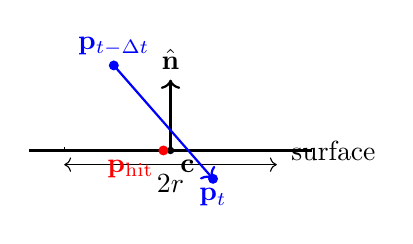
\begin{tikzpicture}[scale=0.9]
\draw[thick] (-2,0) -- (2,0);
\node at (2.3,0) {surface};
\draw[->, thick] (0,0) -- (0,1) node[above] {$\hat{\mathbf{n}}$};
\fill (0,0) circle (1.5pt) node[below right] {$\mathbf{c}$};
\draw[dashed] (-1.5,0) -- (-1.5,0.05);
\draw[<->] (-1.5,-0.2) -- (1.5,-0.2) node[midway,below] {$2r$};
\fill[blue] (-0.8,1.2) circle (2pt) node[above] {$\mathbf{p}_{t-\Delta t}$};
\fill[blue] (0.6,-0.4) circle (2pt) node[below] {$\mathbf{p}_{t}$};
\draw[->, blue, thick] (-0.8,1.2) -- (0.6,-0.4);
\fill[red] (-0.1,0) circle (2pt) node[below left, red] {$\mathbf{p}_\text{hit}$};
\end{tikzpicture}
\caption{Swept-plane collision test. The segment
$\mathbf{p}_{t-\Delta t}\to\mathbf{p}_t$ crosses the plane; the
crossing point must lie within radius $r$ of the centre for the hit
to register.}
\label{fig:collision}
\end{figure}

To prevent re-triggering while the stick lingers against the surface,
each controller maintains an \texttt{engaged} set of instruments it
is currently in contact with. An instrument is removed from the set
only when the tip has receded more than 2\,cm back from the plane
($d_\text{curr}>0.02$), at which point another crossing may fire a
new hit. A 90\,ms per-instrument cooldown guards against spurious
double triggers.

Because the plane is defined in \emph{instrument-local space} and
transformed to world every frame with the instrument's world matrix,
the test is orientation-agnostic: cymbals tilted in two axes, rack
toms tilted forward, or the bass drum facing horizontally toward the
player all use the same code path.

\subsection{Particle system}

Hit feedback is reinforced by a pre-allocated ring buffer of 400
point-sprite particles, rendered with vertex colours and additive
blending. A hit emits between 14 and 40 particles (scaled by
velocity) at the contact point. Velocities are split into a normal
component (along $\hat{\mathbf{n}}$, pushing the spray off the
surface) and a tangential component distributed uniformly in the
plane. The result is that cymbal hits spray sideways along the
edge, while drum hits puff upward off the head. Gravity and a
tangential drag term decelerate the particles into realistic arcs.

\subsection{Internal audio synthesis}

The headset-side audio path uses the Web Audio API. A master bus
feeds a \texttt{DynamicsCompressorNode} and then
\texttt{audioContext.destination}, giving predictable loudness. Each
hit creates a fresh voice graph consisting of oscillators, filtered
noise buffers, and a velocity-scaled gain, all routed through a
\texttt{StereoPannerNode} whose pan value is the hit's $x$ coordinate
clamped to $[-1,1]$.

Synthesis recipes broadly match those in the Pd patch
(section~\ref{sec:pd}) but are implemented imperatively rather than
as a dataflow graph. Their purpose is immediate, low-latency feedback
in the headset --- the Pd engine is the production path.

% ----------------------------------------------------------------
\section{Bridge Server}

The bridge (\texttt{bridge/index.js}) is 130~lines of Node.js. It
runs Express for an \texttt{/status} JSON endpoint, Socket.IO for
browser communication, and the \texttt{osc} package for
Pure~Data. Three event handlers cover the entire behaviour:

\begin{itemize}[leftmargin=2em]
    \item \texttt{drumHit} from the VR client is broadcast to
          spectators (for visual mirroring) \emph{and} translated
          into an OSC packet \texttt{/drum/hit} with arguments
          \texttt{(instrument,\,velocity,\,x,\,y,\,z)} sent to
          \texttt{127.0.0.1:8000}.
    \item \texttt{xrPose} is relayed to other clients so the desktop
          mirror can update its camera and ghost-controller meshes.
    \item \texttt{disconnect} of the VR client triggers an
          \texttt{xrSessionEnd} broadcast so spectators reset to
          their default view.
\end{itemize}

Pose data is sent every other frame (\textasciitilde 36\,Hz) via
\texttt{socket.volatile.emit}, which drops messages rather than
buffering them if the link saturates. This keeps spectator latency
bounded even on flaky Wi-Fi.

% ----------------------------------------------------------------
\section{Pure Data Patch and the Dataflow Paradigm}
\label{sec:pd}

Pure~Data is a \emph{visual dataflow language} for real-time audio and
multimedia. Programs are \emph{patches} consisting of boxes (object
invocations) connected by cords (edges) through which data flows.
There are two fundamental rates: \emph{message rate}, where events
propagate eagerly on demand, and \emph{audio rate}, where 64-sample
vectors flow at a constant $44\,100/64 \approx 689$\,Hz through
objects whose names end in a tilde. The distinction is visible in the
patch: audio cords are drawn thicker.

This project's patch, \texttt{pd/drumset.pd}, follows a classic three-
stage dataflow pipeline: \emph{input}, \emph{voicing}, \emph{mix}.

\subsection{Input and dispatch}

The top of the canvas demultiplexes incoming OSC:

\begin{lstlisting}[language=puredata]
[netreceive -u -b 8000]           ; UDP listener on port 8000
         |
[oscparse]                        ; raw bytes -> typed list
         |
[route /drum/hit]                 ; drop any non-hit messages
         |
[unpack s f f f f]                ; name, velocity, x, y, z
 |   |   |   |   |
 |   |   [s hit-x] [s hit-y] [s hit-z]
 |   |
 +---+--> [pack s f] --> [route bassdrum snare hitom ...]
                                    |   |   |   |  ...
                              [s fire-bassdrum] ...
\end{lstlisting}

\texttt{[unpack]} fires its outlets right-to-left, which means the
$z$, $y$, $x$, and velocity values are published to their respective
\texttt{[s]} buses \emph{before} the instrument symbol reaches
\texttt{[route]}. By the time a voice's \texttt{[r fire-...]} fires,
all context is already latched. This ordering guarantee is a hallmark
of Pd's cold/hot inlet semantics and is the reason no explicit
synchronisation primitives are required.

\texttt{[pack s f]} recombines the instrument name and velocity into
a two-element list. When \texttt{[route]} matches a name, it strips
that name and outputs the remaining list --- a single float, the
velocity --- through the matched outlet. Each voice therefore
receives the velocity through a single \texttt{[r fire-<name>]}
receive, with no additional wiring needed.

\subsection{Sample-based voicing}

The production audio engine is \emph{sample-based}, not synthesised.
Each voice plays back one or more pre-recorded WAV files triggered by
velocity. Two abstraction files implement the two voice flavours:

\begin{itemize}[leftmargin=2em]
    \item \texttt{voice-multi.pd} --- a \textbf{three-layer
          velocity-crossfaded} player used for the bass drum, snare,
          and hi-hat. Three recordings of the same drum at soft,
          medium, and hard intensity play \emph{simultaneously}, each
          weighted by a factor derived from the incoming velocity so
          that the three weights sum to unity.
    \item \texttt{voice-single.pd} --- a single-sample player used
          for the three toms and the two cymbals. One recording is
          scaled linearly by the incoming velocity.
\end{itemize}

Abstractions in Pd take creation-time arguments: inside
\texttt{voice-multi.pd} every reference to \texttt{\$1} is substituted
at load time by the argument passed in the parent. Instantiating
\texttt{[voice-multi bassdrum]} in the main patch therefore resolves
to a voice that listens on \texttt{[r fire-bassdrum]} and reads the
arrays \texttt{bassdrum-soft}, \texttt{bassdrum-med},
\texttt{bassdrum-hard}.

The velocity-to-weight mapping is a pair of tent functions and their
midpoint complement (figure~\ref{fig:xfade}). For an incoming velocity
$v\in[0,1]$,

\begin{align*}
w_\text{soft}(v) &= \max(0,\; 1 - 2v), \\
w_\text{med} (v) &= \min(2v,\; 2(1-v)), \\
w_\text{hard}(v) &= \max(0,\; 2v - 1).
\end{align*}

$w_\text{soft}$ peaks at $v=0$ and falls linearly to $0$ at $v=0.5$;
$w_\text{hard}$ is its mirror; $w_\text{med}$ peaks at $v=0.5$ and
falls linearly to $0$ at both ends. The three curves always sum to
exactly $1$, preserving loudness across the velocity range while the
\emph{timbre} morphs smoothly between the three recordings --- the
crucial property that distinguishes multi-sampling from simple
gain-scaling. A real drum struck softly does not merely produce a
quieter version of its hard hit; the spectral envelope changes too,
and the three recordings capture exactly those changes.

\begin{figure}[h]
\centering
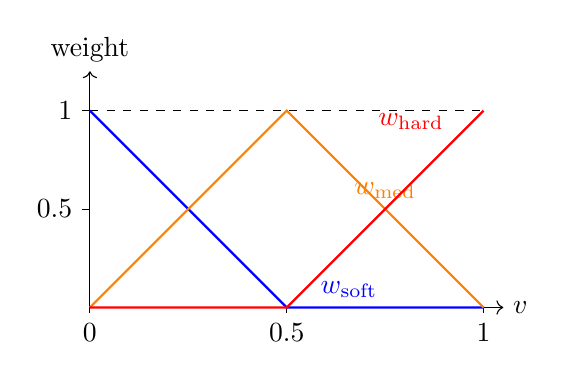
\begin{tikzpicture}[xscale=5, yscale=2.5]
\draw[->] (0,0) -- (1.05,0) node[right] {$v$};
\draw[->] (0,0) -- (0,1.2) node[above] {weight};
\draw[dashed] (0,1) -- (1,1);
\foreach \x in {0, 0.5, 1} {
    \draw (\x,0) -- (\x,-0.03) node[below] {$\x$};
}
\foreach \y in {0.5, 1} {
    \draw (0,\y) -- (-0.02,\y) node[left] {$\y$};
}
\draw[blue,  thick] (0,1) -- (0.5,0) -- (1,0) node[pos=0.12,above right] {$w_\text{soft}$};
\draw[orange,thick] (0,0) -- (0.5,1) -- (1,0) node[pos=0.5,above] {$w_\text{med}$};
\draw[red,   thick] (0,0) -- (0.5,0) -- (1,1) node[pos=0.85,above left] {$w_\text{hard}$};
\end{tikzpicture}
\caption{Three-layer velocity crossfade weights. The curves form a
partition of unity over $[0,1]$, so the combined loudness is
constant while timbre morphs between the three recordings.}
\label{fig:xfade}
\end{figure}

\subsubsection*{Sample sources}

Fourteen WAV files live in \texttt{pd/samples/}. The multisample
layers for bass/snare/hi-hat come from MPC-Tutor's
\emph{8~Layer Drum Kit Tutorial} pack (the kit ships with eight
MIDI-velocity layers; the patch uses layers $31$, $79$, and $127$ for
soft/medium/hard). The single-sample drums come from the
\emph{99Sounds 99~Drum~Samples~I} pack, one acoustic recording per
drum. Both sources are distributed free of charge for non-commercial
use.

\subsubsection*{Loading}

At patch open, a single \texttt{[loadbang]} fires a chained message
containing fourteen comma-separated \texttt{read -resize} commands at
one \texttt{[soundfiler]} object. The receiving
\texttt{[table \textit{name} 100]} declarations provide the target
arrays; \texttt{soundfiler}'s \texttt{-resize} flag expands each array
to fit its source file. Load is synchronous and completes in well
under a second for the 14-file set.

\subsection{Master bus}

All voices \texttt{throw\~{}} to the shared buses \texttt{mix-L} and
\texttt{mix-R}. These are audio-rate send/receive pairs; Pd sums the
contributions automatically. At the bottom of the canvas,
\texttt{catch\~{}} objects retrieve the mixed signal, a master trim
gain scales it, a \texttt{clip\~{} -0.98 0.98} pair provides a cheap
soft limit against inter-sample peaks, and \texttt{dac\~{} 1 2}
outputs to the first two channels of the audio interface.

\subsection{Why dataflow matters here}

The patch is \emph{textually} larger than the equivalent Web Audio
code but \emph{conceptually} smaller: there is no sequencing, no
ordering of function calls, no shared mutable state to reason about.
Each voice is an island whose wiring visibly constrains what it can
do. Editing the patch while it is playing is safe --- changes to a
message box or a filter frequency take effect on the next sample
block, with no restart. This liveness is one of the two qualities
that distinguish dataflow languages for multimedia from imperative
ones.

% ----------------------------------------------------------------
\section{Spectator Mirror}

A non-trivial part of the system is that the desktop browser renders
a live \emph{mirror} of the VR session, useful for demos, recording,
and debugging without constantly swapping the headset.

The mechanism is shared-codebase: both clients load the same
\texttt{main.js}. A boolean \texttt{isSpectator} starts \texttt{true}
and flips on \texttt{renderer.xr.addEventListener('sessionstart', ...)}.
While the VR client is presenting, it publishes a compact pose
message every other frame:

\begin{lstlisting}[language=JavaScript]
socket.volatile.emit('xrPose', {
    cam:  { px, py, pz, qx, qy, qz, qw },   // headset pose
    ctrl: [ctrl0Pose, ctrl1Pose]            // controller poses
});
\end{lstlisting}

The spectator copies those values directly into its
\texttt{THREE.PerspectiveCamera} and two translucent ``ghost''
drumstick meshes, so it sees the VR user's viewpoint plus their hand
positions. Drum hits are mirrored too: each hit triggers a
\texttt{drumHitFeedback} broadcast that the spectator uses to replay
the visual flash, head flex, and particle burst --- but deliberately
not the sound, which stays on the VR side.

% ----------------------------------------------------------------
\section{Building and Running}

\subsection{Prerequisites}

\begin{itemize}[leftmargin=2em]
    \item Node.js 18 or newer on the host PC.
    \item Pure Data vanilla $\geq 0.50$ (no externals required).
    \item A Pico~4 headset on the same Wi-Fi network as the PC, with
          Guardian/boundary configured and the browser set to allow
          WebXR.
\end{itemize}

\subsection{One-time setup}

\begin{lstlisting}[language=bash]
npm run install:all   # installs root + frontend + bridge deps
\end{lstlisting}

\subsection{Running the system}

\begin{enumerate}[leftmargin=2em]
    \item \texttt{npm start} in the repo root launches Vite (HTTPS
          \texttt{:5173}) and the bridge (\texttt{:3000}) concurrently.
    \item Open \texttt{pd/drumset.pd} in Pure~Data and enable DSP
          (Ctrl-/). If the bridge is already running, the terminal
          should show \texttt{[OSC] Ready -> 127.0.0.1:8000}; if Pd is
          now listening on 8000, hits will be synthesised.
    \item On the PC, open \texttt{https://localhost:5173} and accept
          the self-signed certificate. This window is the spectator.
    \item On the Pico, open \texttt{https://<PC-IP>:5173}, accept the
          certificate, and press ``Enter~VR''. Play.
\end{enumerate}

\subsection{Verification}

\texttt{http://localhost:3000/status} returns a small JSON object
describing whether a VR session is connected, the number of
Socket.IO clients, and the OSC target. A quick end-to-end sanity check
is to press a controller trigger without aiming: it should produce
an audible hit from both the headset (Web Audio) and the PC
speakers (Pd), and a matching visual flash in the spectator window.

% ----------------------------------------------------------------
\section{Performance Notes}

The target is a stable 72\,Hz on the Pico~XR2 Gen\,1. Choices made
with that budget in mind:

\begin{itemize}[leftmargin=2em]
    \item The entire scene has $\approx 2\,500$ triangles and
          $\approx 30$ draw calls. Environment IBL is pre-rendered
          once at startup so it imposes no per-frame cost.
    \item Particles are a single 400-element ring buffer drawn as
          one \texttt{THREE.Points} object, not as per-particle
          meshes.
    \item \texttt{Socket.IO} pose messages are emitted as
          \texttt{volatile}, meaning the client drops rather than
          queues them if the link is congested. This avoids
          head-tracking stutter cascading into network latency.
    \item The environment map and the platform are omitted during
          VR presentation (\texttt{scene.background = null}) both
          for passthrough compatibility on the Pico browser and to
          eliminate a full-screen fill.
\end{itemize}

% ----------------------------------------------------------------
\section{Limitations and Future Work}

\paragraph{Fully multisampled toms and cymbals.}
The bass drum, snare, and hi-hat are three-layer velocity-crossfaded;
the three toms and two cymbals are single-sample. Bringing the latter
group up to three-layer multisampling would complete the engine, but
requires a multisampled kit that covers toms and cymbals --- harder
to source than multisampled shells alone. The patch is structured to
make this a one-line change per voice: replacing
\texttt{[voice-single hitom]} with \texttt{[voice-multi hitom]} and
dropping three new WAV files into \texttt{pd/samples/} is all that is
needed.

\paragraph{Convolution reverb.}
A convolution impulse response loaded into \texttt{[partconv\~{}]} on
the master bus would add realistic room ambience. The current master
chain ends in a soft clip; slotting a wet/dry reverb stage between
the catch and the limiter is mechanical.

\paragraph{Hand tracking.}
The Pico~4 supports hand tracking, but the current frontend only
consumes controller input. Extending \texttt{tickCollision} to
additionally sweep from finger-tip joints would let users play
without holding the controllers.

\paragraph{Physical cymbal dynamics.}
Cymbals already wobble angularly on hit via a spring-damped model
(spring constant $k=22$, damping $c=3.5$). The drum shells, by
contrast, only apply an axial compression. A displacement-mapped
drum-head shader that ripples outwards from the contact point would
add another order of visual realism for negligible GPU cost.

\paragraph{Haptics refinement.}
Current haptic feedback is a single \texttt{pulse(intensity, ms)}
call on the gamepad's haptic actuator. A velocity-shaped pulse
(e.g.\ a short burst followed by a slower decay for bass hits) would
better convey stick weight.

% ----------------------------------------------------------------
\section{Conclusion}

MR~Drumset composes three very different programming paradigms into
a single interactive instrument: imperative 3D scene-graph code on
the frontend, event-driven JavaScript on the Node bridge, and
visual-dataflow programming in Pure~Data. The collision layer
demonstrates that correctness in VR interaction comes from modelling
surfaces as proper geometric entities --- planes with centres,
normals, and radii --- not as bounding-sphere approximations. The Pd
patch demonstrates, in turn, that an entire audio engine can be
expressed as a small, readable graph whose structure \emph{is} its
documentation.

% ----------------------------------------------------------------
\section*{References}
\addcontentsline{toc}{section}{References}

\begin{itemize}[leftmargin=2em]
    \item Three.js documentation. \url{https://threejs.org/docs/}
    \item WebXR Device API. W3C Recommendation.
          \url{https://www.w3.org/TR/webxr/}
    \item M. Puckette. \emph{Pure Data}. In Proc.\ International
          Computer Music Conference, 1996.
    \item M. Puckette. \emph{The Theory and Technique of Electronic
          Music}. World Scientific, 2007.
          \url{http://msp.ucsd.edu/techniques.htm}
    \item Web Audio API. W3C Recommendation.
          \url{https://www.w3.org/TR/webaudio/}
    \item Open Sound Control 1.0 specification.
          \url{https://opensoundcontrol.stanford.edu/spec-1_0.html}
\end{itemize}

\end{document}
